\documentclass{article}
\usepackage{tikz}
\usepackage{amsmath,amssymb}

\begin{document}

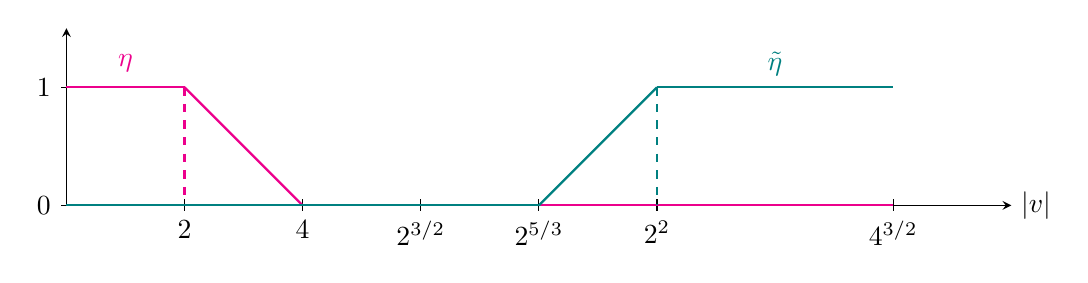
\begin{tikzpicture}[scale=1.5]
    % Axes
    \draw[-stealth] (0,0) -- (8,0) node[right] {$|v|$};
    \draw[-stealth] (0,0) -- (0,1.5);
    
    % Vertical grid lines with labels
    \draw (1,0.05) -- (1,-0.05) node[below] {$2$};
    \draw (2,0.05) -- (2,-0.05) node[below] {$4$};
    \draw (3,0.05) -- (3,-0.05) node[below] {$2^{3/2}$};
    \draw (4,0.05) -- (4,-0.05) node[below] {$2^{5/3}$};
    \draw (5,0.05) -- (5,-0.05) node[below] {$2^{2}$};
    \draw (7,0.05) -- (7,-0.05) node[below] {$4^{3/2}$};
    
    % Horizontal grid lines with labels
    \draw (0.05,1) -- (-0.05,1) node[left] {$1$};
    \draw (0.05,0) -- (-0.05,0) node[left] {$0$};
    
    % Function η (magenta)
    \draw[magenta, thick] (0,1) -- (1,1);
    \draw[magenta, thick, dashed] (1,1) -- (1,0);
    \draw[magenta, thick] (1,1) -- (2,0);
    \draw[magenta, thick] (2,0) -- (7,0);
    
    % Function η̃ (teal)
    \draw[teal, thick] (0,0) -- (4,0);
    \draw[teal, thick] (4,0) -- (5,1);
    \draw[teal, thick, dashed] (5,1) -- (5,0);
    \draw[teal, thick] (5,1) -- (7,1);
    
    % Labels for the functions
    \node[magenta] at (0.5,1.2) {$\eta$};
    \node[teal] at (6,1.2) {$\tilde{\eta}$};
\end{tikzpicture}

\end{document}